
\documentclass{standalone}
\usepackage[svgnames]{xcolor}
\usepackage{pgfplots}
\pgfplotsset{compat=newest}
\usepackage[sfdefault]{FiraSans}
\usepackage{FiraMono}
\renewcommand*\familydefault{\sfdefault}
\begin{document}
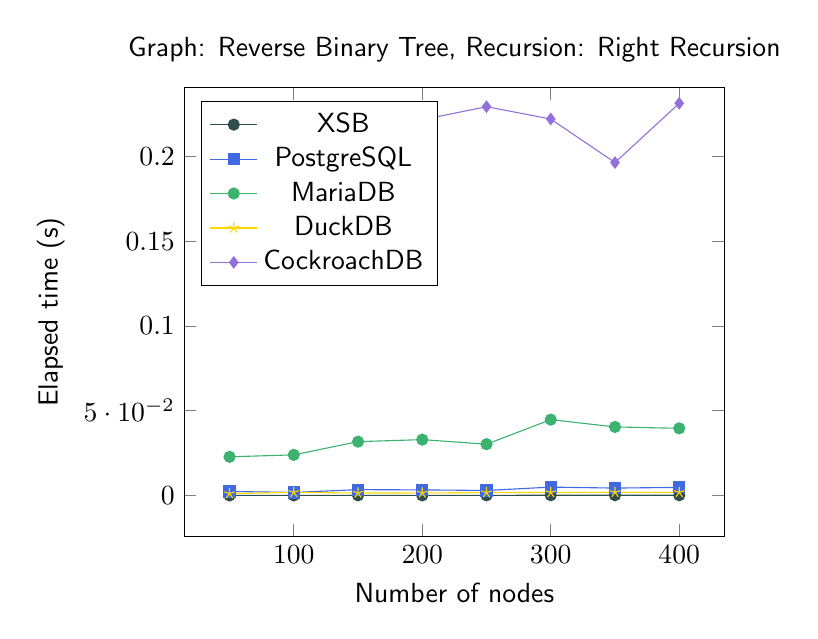
\begin{tikzpicture}
    \begin{axis}[
        title={Graph: Reverse Binary Tree, Recursion: Right Recursion},
        xlabel={Number of nodes},
        ylabel={Elapsed time (s)},
        legend pos={north west},
        ymax=0.24035587498219685
    ]
    \addplot+[DarkSlateGray, mark options={color=DarkSlateGray}] coordinates {(50,2.1409988403320322e-05) (100,3.4189224243164064e-05) (150,6.546974182128911e-05) (200,6.55651092529297e-05) (250,6.494522094726565e-05) (300,0.0001431941986083986) (350,0.0001389503479003908) (400,0.0001390457153320312)};
\addlegendentry{XSB}
\addplot+[RoyalBlue, mark options={color=RoyalBlue}] coordinates {(50,0.0023925666115246712) (100,0.0017829747986979783) (150,0.003448500018566847) (200,0.0032874834025278686) (250,0.0029508166015148165) (300,0.0049337834003381435) (350,0.004365924990270287) (400,0.0047647500061430035)};
\addlegendentry{PostgreSQL}
\addplot+[MediumSeaGreen, mark options={color=MediumSeaGreen}] coordinates {(50,0.02279616678133607) (100,0.023947166593279688) (150,0.03173815819900483) (200,0.03293651659041643) (250,0.03024411640362814) (300,0.04471803319174796) (350,0.04041817479301244) (400,0.039591625006869434)};
\addlegendentry{MariaDB}
\addplot+[Gold, mark options={color=Gold}] coordinates {(50,0.0011092334054410458) (100,0.0018643916002474726) (150,0.001440374623052776) (200,0.0015039166086353362) (250,0.001682233205065131) (300,0.001744375191628933) (350,0.0018665168201550842) (400,0.0018635588116012515)};
\addlegendentry{DuckDB}
\addplot+[MediumPurple, mark options={color=MediumPurple}] coordinates {(50,0.21410316680558025) (100,0.20722194998525084) (150,0.20246655840892344) (200,0.22154865841148422) (250,0.22927037479821594) (300,0.2219779831939377) (350,0.19630913318833337) (400,0.23127183319302275)};
\addlegendentry{CockroachDB}

    \end{axis}
\end{tikzpicture}
\end{document}
